\documentclass{standalone}
%\usepackage{amsmath}\usepackage{lmodern}      % Matches the MathJax default (Latin Modern)
%\usepackage[T1]{fontenc}  % Ensures proper character encoding
\usepackage{tikz}
\usetikzlibrary{positioning, arrows.meta, calc}

% Document metadata (Safe to keep in preamble, standalone will skip them during crop)
\title{Chapter 03 — section 04 — diagram 07}
\author{0im}
\date{2026}

\begin{document}
    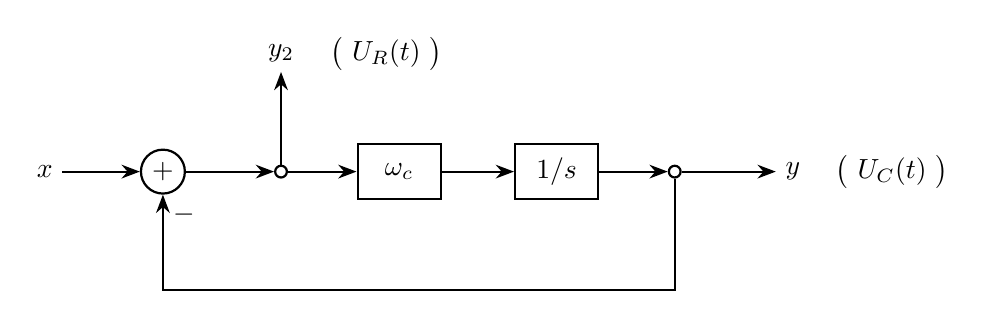
\begin{tikzpicture}
    [
        on grid, 
        node distance=1.5cm and 1.5cm, % Fixed: Added explicit cm units
        block/.style={draw, rectangle, minimum height=2em, minimum width=3em, thick},
        sum/.style={draw, circle, inner sep=2pt, thick},
        branch/.style={draw, circle, inner sep=1.5pt, thick}
    ]
        % =========================================================================
        % NODES
        % =========================================================================
        % --- Row 1 ---
        \node (x) {$x$};
        \node [sum, right=of x] (sum1) {$+$};
        \node [branch, right=of sum1] (branch1) {};
        \node [block, right=of branch1] (cutoff1) {$\omega_c$};
        \node [block, right=2cm of cutoff1] (int1) {$1/s$};
        \node [branch, right=of int1] (branch2) {};
        \node [right=of branch2] (y) {$y$};
        \node [right=0.42cm of y, anchor=west] (UC) {$ \bigl( \ U_C (t) \ \bigr) $};
        % --- Row 2 ---
        \node [below=of sum1] (blank1) {};
        \node [below=of branch2] (blank2) {};
        % --- Row 0 ---
        \node [above=of branch1] (y2) {$y_2$};
        \node [right=0.5cm of y2, anchor=west] (UR) {$ \bigl( \ U_R (t) \ \bigr) $};
        
        % =========================================================================
        % PATHS
        % =========================================================================
        % --- HORIZONTAL ---
        \draw [-Stealth, thick] (x.east) -- (sum1.west);
        \draw [-Stealth, thick] (sum1.east) -- (branch1.west);
        \draw [-Stealth, thick] (branch1.east) -- (cutoff1.west);
        \draw [-Stealth, thick] (cutoff1.east) -- (int1.west);
        \draw [-Stealth, thick] (int1.east) -- (branch2.west);
        \draw [-Stealth, thick] (branch2.east) -- (y.west);
        % --- VERTICAL ---
        \draw [-Stealth, thick] (branch1.north) -- (y2.south);
        % --- ANGLED ---
        \draw [-Stealth, thick]
            (branch2.south) -- (blank2.center) -- (blank1.center) -- (sum1.south)
            node [anchor=north west] {$-$};
    \end{tikzpicture}
\end{document}